\chapter{Ingénierie Système}

\section{Analyse Fonctionelle}

\subsection{Diagramme Pieuvre}

Le diagramme pieuvre permet de mettre en évidence rapidement la fonction principale du système et les principales contraintes qui s'appliquent sur le système. Ce dernier est représenté par l'ovale central et l'ensemble des éléments extérieurs ayant une influence sont matérialisés tout autour. Les différentes relations sont appelées les fonctions de contraintes qui naissent d'une contrainte imposée par un élément extérieur « météo », de l'existence d'un produit déjà existant « un autre drone émettant des ondes » ou encore d'une exigence particulière de l'utilisateur voire de la présence de normes et de législations, de limitations lié au budget ou du type d'alimentation énergétique nécessaire.


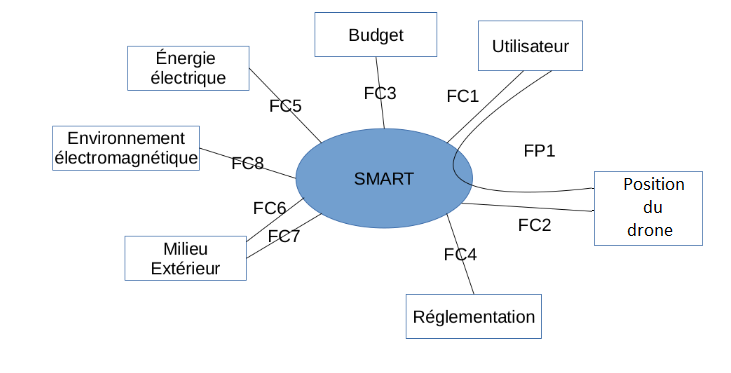
\includegraphics[width=0.90\textwidth]{Diagramme_pieuvre_corr.png}
\captionof{figure}{Diagramme pieuvre}


\subsection{Diagramme FAST}

Ce diagramme  présente la  manière de penser et d'agir. Le diagramme FAST se construit de gauche à droite, dans une logique du pourquoi au comment. On développe les fonctions de service du système en fonctions techniques. On choisit des solutions pour construire finalement notre système. On a mentionné les fonctions techniques chacune  à part pour trouver la solution convenable qui nous permet à la fin la réalisation finale du système. En utilisant des outils et méthodes déjà existant, on a trouvé des solutions qui satisfont les fonctions demandés.
L’antenne goniomètre était l’une des solutions les moins chères pour la détection du drone, à condition d’avoir au minimum deux antennes pour préciser la position et la vitesse du drone. Dès la détection du drone, il sera alors possible de déterminer sa position, d'enregistrer cette position via un logiciel dédié (MATLAB)

~\\

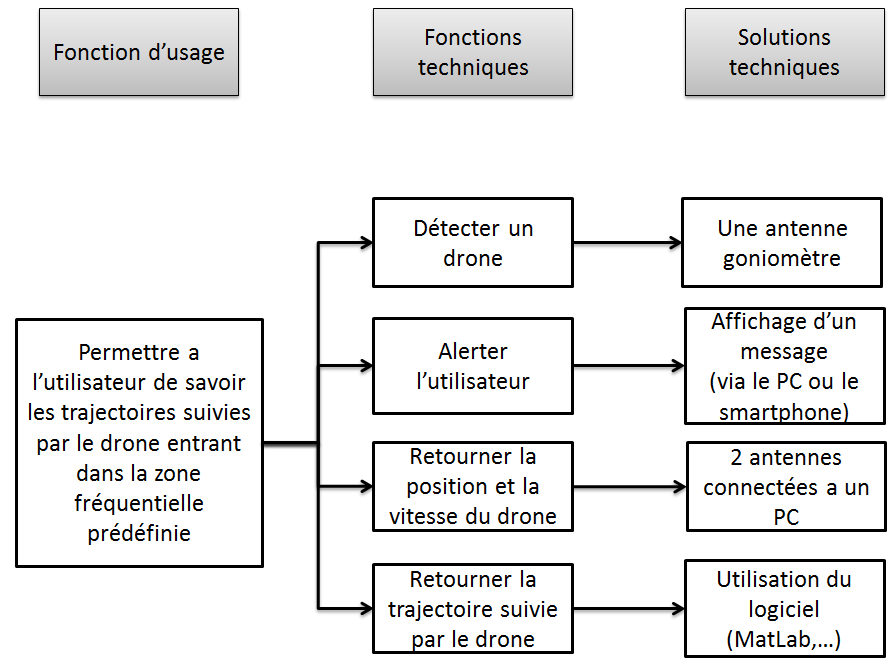
\includegraphics[width=1\textwidth]{FAST.png}
\captionof{figure}{Diagramme pieuvre}

%%% Local Variables: 
%%% mode: latex
%%% TeX-master: "../rapport"
%%% End: 